\chapter{Overview of the DSS-63 and IRAM 30m antennas} % (fold)
\label{cha:overview_of_the_dss_63_and_iram_30m_antennas}

In this appendix we will have an overview of the DSS-63 and IRAM 30m
antennas, together with their observing modes and scientific storage
needs, in order to better understand the decisions taken when creating
the RADAMS ---see chapter~\ref{cha:radams}---.

\section{DSS-63} % (fold)
\label{sec:dss_63}

The DSS-63 is one of the antennas at the Madrid Deep Space
Communications Complex. Three Deep Space Communications Complexes
(DSCCs) where created by NASA in the late 50’s, and where located at
Canberra (Australia), Madrid (Spain) and Goldstone (USA), in order to
allow for continuous monitoring of the incoming data from
Earth-orbiting and interplanetary spacecraft missions, as well as
radio and radar astronomy observations for the exploration of the
Solar System and the Universe. The combined operation of the three
DSCCs is what it is known as the Deep Space Network (DSN), which is
managed by the Jet Propulsion Laboratory (JPL).

Of all the time devoted for astronomical observations, around 3\% of
the time at the Canberra and Madrid stations (up to 260 hours per
antenna) is available to Host-Country astronomers. The organisation
responsible for the scheduling of this time at Madrid DSCC is the
Laboratorio de Astrofísica Espacial y Física Fundamental (LAEFF) of
the Instituto Nacional de Técnica Aeroespacial (INTA), by arrangement
with NASA.

Each DSCC has at least four operational antennas:

\begin{itemize}
	\item One 26-meter diameter antenna, originally built to
          support the Apollo missions to the Moon, presently used for
          communicating with Earth-orbiting spacecraft.
	
	\item One 34-meter diameter high efficiency antenna (HEF),
          designed around a precision-shaped reflector, for maximum
          signal sensitivity.
	
	\item One 34-meter diameter beam waveguide antenna (BWG),
          based on the HEF design, with five mirrors that reflect radio
          signals along a beam-waveguide tube from the antenna vertex
          to the equipment room, for easier maintenance access.
	
	\item One 70-meter diameter antenna, with the highest
          sensitivity, used for tracking the deepest space missions.
\end{itemize}

Nowadays, Host Country time at the MDSCC is dedicated to perform
spectroscopic observations at K-band (i.e., wavelengths around 1 cm),
with the 70-m DSS-63 antenna.

Table \ref{dss63properties} summarises the main properties for the
DSS-63 antenna, and Table \ref{dss63comparison} compares them with
those from other similar radio telescopes. Figure \ref{dss63image}
shows a picture of the 70-m antenna.

%\begin{table}[tbp]
%\begin{minipage}{\linewidth}
%\caption[DSS-63 antenna, receiver and spectrometer properties]
%{DSS-63 antenna, receiver and spectrometer properties.}
%\begin{smalltabular}{cl} \hline
%\multirow{10}*{\minitab[c]{\textbf{Antenna} \\ 
%\textbf{System}\footnote{HPBW, aperture efficiency, sensitivity and
%pointing accuracy measured at 22GHz, with 40º of elevation}}}
%		& \textbf{Name}: Deep Space Station 63 \\ & \textbf{Diameter}:
%        70 m \\ & \textbf{Type}: parabolic Cassegrain \\ &
%        \textbf{Mount}: azimuth/elevation \\ & \textbf{Latitude}: 40º
%        25’ 52’’ N \\ & \textbf{Longitude}: 04º 14’ 53’’ W \\ &
%        \textbf{Altitude}: 865.5 m \\ &
%        \textbf{HPBW}\footnote{Half-Power Beam Width}: 42’’ \\ &
%        \textbf{Aperture Efficiency ($\eta$)}: 49\% maximum \\ &
%        \textbf{Sensitivity}: 0.7 K/Jy \\ & \textbf{Pointing accuracy}:
%        $\leq$ 10'' \\ \hline \multirow{5}*{\minitab[c]{\textbf{K-band}
%        \\ \textbf{receiver}}} & \textbf{Amplifier type}: cooled HEMT
%        \\ & \textbf{Frequency range}: 18-26 GHz \\ &
%        \textbf{Polarisation}: LCP\footnote{Left Circular Polarisation}
%        or RCP\footnote{Right Circular Polarisation} (default, LCP) \\
%        & \textbf{$\mathbf{T_{sys}}$ (winter)}: 50 K \\ &
%        \textbf{$\mathbf{T_{sys}}$ (summer)}: 75 K \\ \hline
%        \multirow{17}*{\minitab[c]{\textbf{Spectrometers}}} &
%        \textbf{Spaceborne-500}\footnote{This is the correlator
%        currently in used, and superseded the Spectra-Data.}\\ &
%        \textbf{Type}: Digital autocorrelator \\ & \textbf{BW}: 2, 4, 8
%        and 16 MHz\\ & \textbf{Num. channels}: 384\\ &
%        \textbf{Observing mode}: position switching\\ & \\ &
%        \textbf{Spectra-Data}\footnote{The Spectra-Data was the
%        correlator initially used at the facility (from 2001 to 2003),
%        but it is no longer operational.}\\ & \textbf{Type}:
%        Fourier-transform autocorrelator \\ & \textbf{BW}: 1, 2.5, 5
%        and 10 MHz\\ & \textbf{Num. channels}: 256\\ &
%        \textbf{Observing mode}: frequency switching\\ & \\ &
%        \textbf{SAO4K}\footnote{The SAO4K correlator belongs to the
%        Smithsonian Astrophysical Observatory, and is used in the SAMBA
%        survey.}\\ & \textbf{Type}: Digital autocorrelator \\ &
%        \textbf{BW}: 400 MHz\\ & \textbf{Num. channels}: 4096\\ &
%        \textbf{Observing mode}: position switching\\ \hline
%\end{smalltabular}
%\label{dss63properties}
%\end{minipage}
%\end{table}

%\begin{table}[tbp]
%\caption[DSS-63 properties, versus other antennas]
%{DSS-63 properties, versus other antennas; values at 22 GHz.}
%\begin{smalltabular}{ccccc} \hline
%		& & \textbf{Aperture} & & \textbf{Sensitivity} \\
%        \textbf{Telescope} & \textbf{Diameter} & \textbf{efficiency
%        ($\mathrm{\eta_a}$)} & \textbf{Resolution} &
%        \textbf{(K/Jy)}\\[4pt] \hline Effelsberg & 100 m & 29\% & 40’’
%        & 0.8\\ GBT & 100-110 m& 55\% & 34’’ & 1.5\\ Robledo DSS-63 &
%        70 m & 49\% & 42’’ & 0.7\\ \hline
%\end{smalltabular}
%\label{dss63comparison}
%\end{table}

\begin{figure}[tbp]
\begin{center}
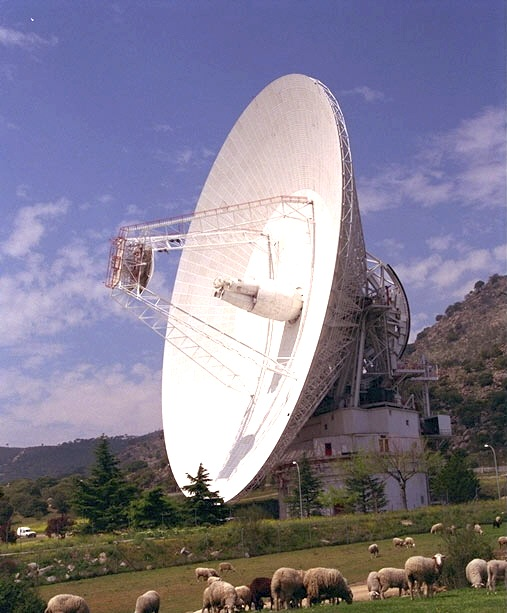
\includegraphics[width=0.75\columnwidth]{fig/DSS-63.jpg}
\caption[DSS-63 70-meter antenna]
{DSS-63 70-meter antenna at Robledo de Chavela, Madrid}
\label{dss63image}
\end{center}
\end{figure}

\subsection{Observations with DSS-63} % (fold)
\label{sub:observations_with_dss_63}

\subsubsection{Spectral observations} % (fold)
\label{ssub:spectral_observations}

The main scientific use of the DSS-63 antenna is the recollection of
spectra. The observing process for a spectrum with this antenna is as
follows:

\begin{description}
	\item[Source selection] First, a target source with a medium
       elevation at the time of observation is selected; extreme
       elevations introduce additional pointing errors and/or
       additional atmospheric effects.
	
	\item[Pointing calibrator selection] Once the source has
       been selected, a strong pointing calibration source near the
       target is chosen; minimisation of antenna motion between
       pointing calibration and the actual observation is desirable.
	
	\item[Pointing calibration] The antenna will be moved up and
       down in elevation, and clockwise and counter-clockwise in
       cross-elevation, around the expected position for the
       pointing calibrator. As the profile for the telescope beam
       conforms to a Gaussian distribution, the data can be fitted
       with a Gaussian, and the pointing error adjusted by
       comparison between the expected position of the calibrator,
       and the fitted Gaussian flux. This correction will be
       applied to the coordinates where the source is expected to
       be.
	
	\item[Focus calibration] The same calibrator can be used to
       calibrate the focus of the instrument, defined as the
       position of the secondary mirror that maximises the power
       collected by the instrument. Again, the profile for the
       focus, when the mirror is moved along its axis, is assumed to
       be Gaussian, and the fit for the maximum provides the focus
       position.
	
	\item[On/Off source observation] Both the source and a
       nearby position with no emissions have to be observed, in
       order to discriminate the contribution from the instrument.
       This is performed either by changing the position of the
       antenna (position switching), or by moving the secondary
       mirror in such a way that the main feed is focused on a
       different region of the sky, with no radio sources (wobbler
       switching). Another possibility is to compare the power of
       the emission from the same source at slightly different
       frequencies, assuming that the antenna and atmospheric noise
       does not change with this frequency switch (frequency
       switching). In the case of the DSS-63, on/off observations
       are performed either by position switching or frequency
       switching.
	
	\item[Atmospheric corrections] The amount of energy received
       by the instrument depends strongly on weather conditions, and
       on the length of the path of the signal through the
       atmosphere. In particular, at cm wavelengths the amount of
       water vapour in the atmosphere is the major contributor to
       atmospheric opacity (a quantity that is proportional to the
       probability of a photon being absorbed after travelling a
       given length in the atmosphere). Measurements of opacity at
       different elevations (tipping curves, or skydips), which
       correspond to different air masses (a measure of the amount
       of atmospheric gas in the line of sight of the instrument),
       are used to fit a curve that provides the atmospheric
       opacity. This is usually done at DSS-63 once per observing
       session and frequency setup.
\end{description}

There are other corrections and calibrations to consider, but most of
them can be obtained from typical values for the instrument and
particular configuration, and do not contribute to illustrate the
observing process with the DSS-63 antenna.

Of particular interest will be parameters such as system temperature
($\mathrm{T_{sys}}$), main beam solid angle ($\mathrm{\Omega_{mb}}$),
aperture efficiency ($\mathrm{\eta_a}$), and the antenna temperature
scale.

The data output of the correlator is a 384-sample autocorrelation
function, which by means of the Fourier transform (Discrete Fourier
Transform, in this case) provides a function proportional to the
power spectrum of the source. The post-processing of the observation,
together with the calibration procedures, will allow us to determine
the actual spectrum scale, and frequencies for the salient features
of the spectrum.

% subsubsection spectral_observations (end)

% subsection observations_with_dss_63 (end)

% section dss_63 (end)

\section{IRAM 30m} % (fold)
\label{sec:iram_30m}

\subsection{Observations with IRAM 30m} % (fold)
\label{sub:observations_with_iram_30m}

% subsection observations_with_iram_30m (end)

% section iram_30m (end)


% chapter overview_of_the_dss_63_and_iram_30m_antennas (end)